\section{Ermittlung der Anforderungen}
\subsection{Ermittlung der Stakeholder}
Bevor mit der Ermittlung der Anforderungen begonnen wird, müssen zuerst die Stakeholder identifiziert werden, die ein allgemeines Interesse an der zu entwickelnden Software, bzw. dem Tool haben. Dabei handelt es sich um Personen, die entweder von dem fertigen Produkt profitieren, oder die später das Produkt zu ihrer täglichen Arbeit einsetzen und daher ein Interesse am Funktionsumfang und der Benutzerfreundlichkeit haben. 

\subsubsection{Analyse der Stakeholder}
Im Falle des Business-Transformation-Trackers wurde folgende Stakeholder ermittelt:
\begin{itemize}
    \item[] \emph{Oberes Management:} Das obere Management der adesso orange AG ist der Auftraggeber für das Entwicklungsprojekt und hat daher besonderes Interesse in der erfolgreichen Fertigstellung des Projekts und der Produktivsetzung des Systems, um mit dieser Wertschöpfung zu generieren. Dazu kommt, dass das Ziel der Entwicklung die Unterstützung der Mitarbeiter in den Projekten ist und sich durch den Einsatz eine Effizienzsteigerung und Qualitätsverbesserung erhofft wird. Dadurch besteht die Möglichkeit der Reputationssteigerung gegenüber potentiellen Kunden und somit einer gesteigerten Nachfrage im Vertrieb, was ebenfalls im besonderen Interesse des Managements liegt. In Persona tritt das obere Management im Entwicklungsprojekt als Bereichsleiter \glqq{}SAP Consulting and Development\grqq{} in Erscheinung.
    \item[] \emph{Mittleres Management:} Die Mitarbeiter der adesso orange AG im mittleren Management fungieren in der Regel in der Rolle eines Abteilungs- oder Projektleiters und haben daher ein besonderes Interesse an dem Funktionsumfang an der zu entwicklenden Software, da sie durch den Funktionsumfang direkt in den Projekten profitieren können. So profitieren sie beispielsweise von einer übersichtlichen Ansicht des gesamten Projekts und können durch Auswertungen besser das Projekt verwalten. Außerdem besitzen die Mitarbeiter des mittleren Managements ein Interesse darin, dass das Tool durch die Mitarbeiter verwendet wird, damit die darin geführten Daten stets auf dem aktuellen Stand sind. 
    \item[] \emph{Senior Consultants:} Senior Consultants sind erfahrene Mitarbeiter von adesso orange und arbeiten in der Regel als Projektleiter in kleineren Projekten oder als Teilprojektleiter in Projekten mit größerem Umfang. Sie haben ein großes Interesse in den Funktionsumfang des BTT und der Aktualität der darin enthaltenden Daten. Dadurch sind sie sehr an der zentralen Datenhaltung, sowie an der Übersichtlichkeit und Benutzerfreundlichkeit der grafischen Oberfläche interessiert, da sie, zusammen mit den Consultants, am intensivsten mit dem Programm arbeiten werden. Dabei stehen die Ziele der Datenkonsistenz und der generellen Verfügbarkeit des BTT im Vordergrund, damit eine reibungslose Arbeit ermöglicht wird.
    \item[] \emph{Consultants:} Die Consultants, bzw. Berater bilden den Kern der Mitarbeiterschaft des auftraggebenden Unternehmens und treten in der Regel als Projektmitarbeiter in Erscheinung. Sie bilden die größte Zielgruppe, da sie am häufigsten mit dem Programm arbeiten werden und dort den Großteil der Datenerfassung durchführen werden. Deshalb ist es vom besonderen Interesse, den Projektmitarbeitern die Arbeit mit dem Produkt möglichst einfach zu machen und besonders auf die Benutzerfreundlichkeit in der Entwicklung zu achten. Dazu kommt, dass es wichtig ist, diese Stakeholdergruppe möglichst in die Entwicklung mit einzubeziehen, um Verbesserungsvorschläge und Ideen in die Anforderungen mit aufzunehmen. 
    \item[] \emph{Entwickler:} Die (SAP-)Entwickler des Auftraggebers spielen nur eine untergeordnete Rolle im Kontext des Business Transformation Tracker, da die Befüllung und Auswertung nicht in ihr Aufgabenfeld gehört. Denkbar sind dennoch Szenarien, in denen sie aufgefordert werden, einzelne Einträge in dem Programm vorzunehmen, zu denen ihre Expertise benötigt wird. Auch besteht ein großes Interesse an Benutzerfreundlichkeit und Übersichtlichkeit, damit auch bei seltener Nutzung der Umgang mit dem Programm nicht schwerfällt.
    \item[] \emph{Kunden:} Weitere Stakeholder sind die Kunden von adesso orange, da diese ebenfalls Berührungspunkte mit dem Programm haben werden, wenn es Teil ihres Transformationsprojekts wird. Sie haben ein besonderes Interesse an der gesteigerten Effizienz und der gesteigerten Qualität ihrer Transformation, da dies für sie eingesparte Ressourcen in Form von weniger Projekttagen, weniger Aufwänden für die Transformation und geringere Wartungskosten im Anschluss durch die gesteigerte Qualität der Prozesse bedeutet. Dazu kommt, dass es dazu kommen kann, dass in größeren Projekten die Mitarbeiter des Kunden ebenfalls in direkten Kontakt mit dem BTT kommen, um bspw. bei der Erfassung der Prozesse zu unterstützen. Dadurch entsteht ein großes Interesse an der Übersichtlichkeit und der Benutzerfreundlichkeit, damit auch bei einmaliger Benutzung das gewünschte Resultat zustande kommt.
\end{itemize}

\subsubsection{Riskobewertung der Stakeholder}
Von den unterschiedlichen Stakeholdern gehen unterschiedliche Risiken im Bezug auf den Erfolg des Produkts aus. So gibt es auf der einen Seite ein unterschiedliches Konfliktpotential, das durch die unterschiedlichen Einflussmöglichkeiten der Stakeholder, verschiedene Probleme im späteren Einsatz des Tools herbeiführen kann. So wäre es zum Beispiel denkbar, dass ein Consultant die Arbeit mit dem BTT verweigert, wenn seine persönlichen Anforderungen, in Form von Benutzerfreundlichkeit, außer Acht gelassen werden, oder, das ein Mitarbeiter des mittleren Managements, in Form eines Projektleiters, den Einsatz von Anfang an gar nicht erst vorsieht, wenn dieser den Standpunkt vertritt ist, dass das Tool keinen Mehrwert bietet, wenn seine Anforderungen an das Programm, beispielsweise in Form von Verfügbarkeit und Zuverlässigkeit, nur unzulänglich erfüllt werden.
\begin{figure}[ht]
    \centering
    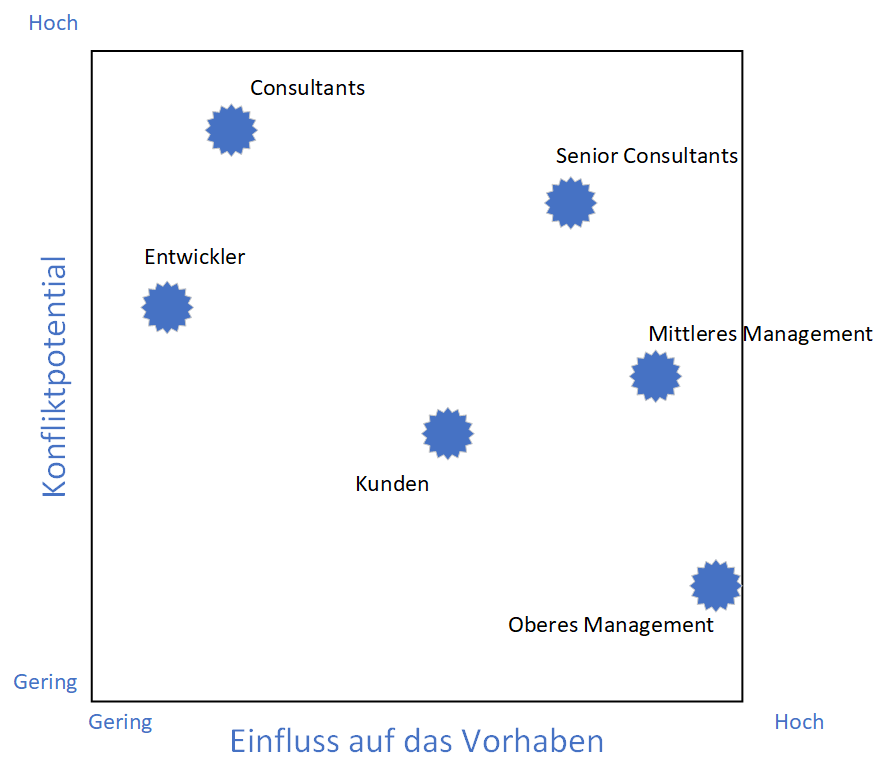
\includegraphics[scale=0.67]{Bilder/stakeholderRisiko.png}
    \caption[Risikobewertung der Stakeholder]{Subjektive Risikobewertung der genannten Stakeholder}
\end{figure}
Dieses Konfliktpotential lässt sich umgehen, indem die Personengruppen frühzeit in die Anforderungsermittlung mit eingebunden werden und sie dadurch, im Rahmen der Möglichkeiten, selbst bei der Produktentwicklung mitwirken können. Besonders bei Stakeholdern mit großem Einfluss und hohem Konfliktpotential ist es daher wichtig Maßnahmen zu definieren, wodurch dieses gesenkt werden kann.\footcite[Vgl.][S. 504 f.]{balzert}

\subsection{Erhebung der Anforderungen}
\subsubsection{Informationen durch den Auftraggeber}
Zur Ermittlung der Anforderungen fanden mehrere Gespräche mit dem Auftraggeber statt, in denen zum einen auf den aktuellen Ist-Zustand eingegangen, und zum anderen Ideen und Umsetzungsvorschläge besprochen wurden. Diese Informationen sind bereits in dem vorangegangenen Kapitel \ref{kap:istzustand} in der Problemstellung und in der Beschreibung des Ist-Zustandes untergebracht und werden nun genutzt, um daraus die Anforderungen an das in Auftrag gegebene Programm zu entwickeln. Während des Entwicklungsprozesses besteht ein enger Kontakt zu dem Auftraggeber, wodurch auftretende Rückfragen schnell beantwortet werden können. 

\subsubsection{Befragung im Unternehmen}
\label{kap:Umfrage}
Um von möglichst vielen Stakeholdern Anforderungen an eine Neuentwicklung des Business Transformation Trackers zu erhalten, wurde mit den Mitarbeitern der adesso orange, die bereits mit der aktuellen Umsetzung des BTT, bzw. seinem Vorgänger, gearbeitet haben, eine Onlineumfrage durchgeführt. Ziel der Befragung war es zum einen, das generelle Meinungsbild der Mitarbeiter zu dem BTT zu erfassen und zum anderen mögliche Verbesserungsvorschläge und Ideen der Stakeholder aufzugreifen, um daraus Anforderungen an einen Neuaufbau des BTT zu entwickeln. Die Umfrage richtet sich dabei an alle internen Stakeholder, das heißt an die Mitarbeiter des oberen und mittleren Managements, an die Senior Consultants, Consultants und Entwickler. Dadurch soll ein möglichst breites Bild entstehen, dass alle Interessen abdeckt, sodass kein Stakeholder vernachlässigt wird.\\Die Umfrage wurde mit der Online-Plattform \glqq{}Microsoft Teams\grqq{} umgesetzt, das Bestandteil der im Unternehmen eingesetzten Softwaresuite \glqq{}Microsoft 365\grqq{} ist. Die Umfrage wurde anonym durchgeführt, mit der Möglichkeit am Ende freiwillig seine Kontaktdaten anzugeben, um Rückfragen zu den gegebenen Antworten und Vorschlägen zu ermöglichen. In Anhang A sind die einzelnen Fragen der Umfrage, sowie ihre Antwortmöglichkeiten abgebildet. Der Fragenkatalog bestand aus drei Abschnitten, zuerst allgemeine Fragen zur Person und zur Position im Unternehmen, als Nächstes mit Fragen zur Meinung über den BTT und zum Schluss mit der Möglichkeit Verbesserungsvorschläge und Ideen anzugeben. Um dem Betriebsklima im Unternehmen gerecht zu werden, wurde in der Umfrage auf die förmliche Anrede der Befragten verzichtet.

\subsubsection{Ergebnisse der Umfrage}
Es wurden etwa 15 Mitarbeiter zu der eingangs erwähnten Umfrage eingeladen, die bereits in adesso active transformation -Projekten mitgewirkt haben. Die Befragten hatten eine Woche Zeit, die Umfrage zu beantworten, in diesem Zeitraum wurden acht Antworten abgegeben. Dabei ergab sich, dass die meisten der Befragten bereits viele Erfahrungen im SAP-Umfeld gesammelt haben und bei der adesso orange in einer entsprechenden Position arbeiten. Von den acht Mitarbeitern, die an der Umfrage teilnahmen, sind 4 in der Stellung eines Senior Consultants tätig. Zwei der restlichen Befragten waren jeweils in einer Anstellung darüber und darunter tätig. Fünf der Befragten wurden bereits als Teilprojektleiter oder einer höheren Position in einem adesso active transformation eingesetzt. 
\\Zu dem Meinungsbild über die jetzige Umsetzung des BTT lässt sich sagen, dass es sich zwischen denen, die bereits häufig mit dem BTT gearbeitet haben und denen, die noch eher wenig Kontakt mit hatten, merkbar unterscheidet. Diejenigen, die bereits häufiger mit dem Tool gearbeitet haben, gaben in der Umfrage an, dass sie gerne mit dem BTT arbeiten und auch in der Anwendung gut mit ihm zurechtkommen. Diejenigen, die noch nicht so häufig mit dem Tool in Kontakt kamen, denken eher das Gegenteil. Auffällig ist ebenfalls, dass die meisten der Befragten der Aussage zustimmen, dass der BTT eher mehr belastet, als das er nutzt. Das führt dazu, dass viele der Teilnehmer angaben, dass sie Verbesserungspotenziale im BTT sehen, dieser jedoch im Grunde genommen, ein gutes Mittel zum Ziel ist.\\
In dem Abschnitt der Umfrage, in dem Verbesserungsvorschläge und Ideen angegeben werden konnten, brachten die Befragten zum Ausdruck, dass sie empfinden, dass Geschäftsprozesse zu wenig Beachtung im BTT finden, und dieser zu transaktionsorientiert ausgerichtet ist. Ebenfalls wurde bemängelt, dass der BTT zu wenig als Analysewerkzeug eingesetzt wird und, dass er in seiner jetzigen Implementierung zu unübersichtlich sei, da er aus zu viele Spalten bestehe und diese teilweise redundant zueiander sind. Als Vorschläge für eine Erweiterung des Funktionsumfangs wurde geäußert, dass die Gruppierung nach Prozessen intensiviert werden soll, dass sich gewünscht wird, dass SAP-Buchhaltungsmodule gemeinsam abgebildet werden und, dass an der Übersichtlichkeit, etwa durch Farben oder Feldlisten, gearbeitet werden soll. \emph{Die vollständigen Antworten der Umfrage sind in Anhang B zu finden.}
\\Zusammenfassend lässt sich sagen, dass die Mitarbeiter von adesso orange nicht sonderlich zufrieden mit der jetzigen Umsetzung des Business Transformation Trackers sind. Man bemängelt den Funktionsumfang, sowie die Unübersichtlichkeit des Excel-Spreadsheets, verkennt jedoch nicht, dass das Tool nützlich sein kann und im Grunde genommen ein gutes Mittel für das angestrebte Ziel ist. Das bestärkt die Konzeption einer Neuentwicklung, in der die Wünsche der Mitarbeiter Beachtung finden und diese in die Anforderungen mit aufgenommen werden. 

